\subsection{Prediction View}
\label{sec:prediction}
For a given sentence pair, the model predicts a discrete probability distribution of the three labels (neutral, contradict, and entailment).
%
In the prediction view, as illustrated in Fig.~\ref{fig:predictionView}, a prediction probability is encoded as a point in the barycentric coordinate system of the triangle. In the triangle, the distinct color indicates the region corresponds to different labels. The prediction result for the original sentence pair is represented by the larger yellow circle, whereas smaller grey circles illustrate the perturbed sentence pairs. A density contour of the prediction is computed to emphasis the highly cluttered areas and distinguish the outliers.

To address \textbf{T3}, we need a way to communicate the reassignment of the prediction. As illustrated in (b), we integrate such operation in the prediction review. When press and drag the prediction (represented as circle), the user is presented with the three option (E, N, C) corresponds to the labels. When the user hovers on one of the options, a dotted line is shown to indicate the newly assigned label. The new label is assigned when the user release the mouse, when hovering on the desired label choice.

\begin{figure}[htbp]
\centering
\vspace{-2mm}
 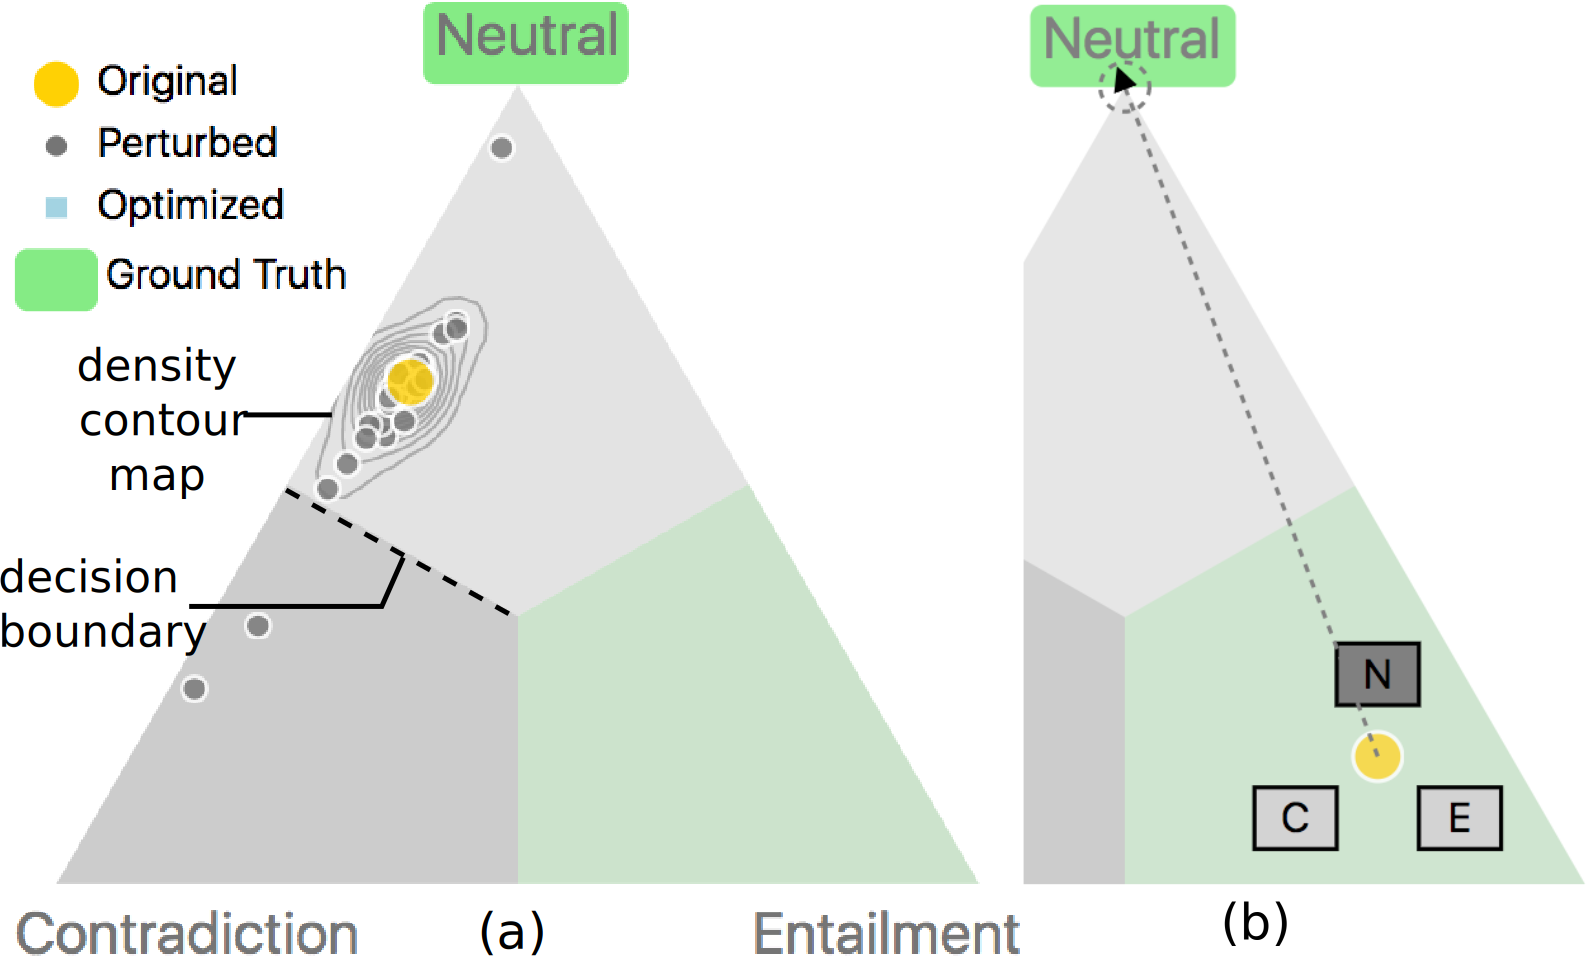
\includegraphics[width=1.0\linewidth]{predictionView}
 \vspace{-2mm}
 \caption{
In the prediction view, the prediction is encoded as a point in the barycentric coordinate system of the triangle shown in (a).
%
The prediction result for the original sentence pair is represented by a larger yellow circle and the prediction of perturbed pairs are illustrated by smaller grey circles.
A density contour of the prediction is computed to emphasize the highly cluttered areas and distinguish the outliers.
As illustrated in (b), the predicted label does not match the ground truth, therefore, we apply a label reassignment operation, which triggers the model update.
% when press and drag the circle (prediction), the user is presented with the three option corresponds to the labels. The dotted line and arrow indicate the newly assigned label.
 }
\label{fig:predictionView}
\end{figure}
